\documentclass[12pt, a4paper]{article}
\usepackage[a4paper, mag=1000, left=2cm, right=1cm, top=2cm, bottom=2cm, headsep=0.7cm, footskip=1cm]{geometry}

\usepackage[utf8]{inputenc}	
\usepackage[russian]{babel}
	
\usepackage{graphicx}
\usepackage{amsmath}
\usepackage{amsfonts}
\usepackage{amssymb}
\usepackage{indentfirst}
\usepackage{wasysym}
\DeclareUnicodeCharacter{04C3}{\khk}
\newcommand{\HRule}{\rule{\linewidth}{0.5mm}}


\begin{document}
\begin{titlepage}
\begin{center}

\textsc{\large РОССИЙСКИЙ ХИМИКО$-$ТЕХНОЛОГИЧЕНСКИЙ УНИВЕРСИТЕТ ИМЕНИ Д.И.МЕНДЕЛЕЕВА}\\
\textsc{\large }\\[2cm]

% Upper part of the page. The '~' is needed because \\
% only works if a paragraph has started.

\includegraphics[width=0.35\textwidth]{img/logo.png}~\\[2cm]

\textsc{\Large Теоретические основы процессов массообмена}\\[0.3cm]

\textsc{ \textbf{Отчёт по лаборатоной работе \textnumero 3}}\\[0.3cm]

% Title
\HRule \\[0.4cm]
{ \large ТЕПЛООБМЕН В ПРОТОЧНОМ АППАРАТЕ С МЕШАЛКОЙ \\[0.4cm] }

\HRule \\[1.5cm]

% Author and supervisor
\noindent
\begin{minipage}[t]{0.6\textwidth}
\begin{flushleft} \large
\emph{Студенты:}\\
Соколова \textsc{A.~Н.} \\
Аганичева \textsc{И.~В.} \\
Мшенская \textsc{В.~А.} \\
Эгембердиев \textsc{М.~Р.} \\
Григорьев \textsc{С.~В.} \\
Киалуэ \textsc{М.~К.} \\
\end{flushleft}
\end{minipage}%
\noindent
\begin{minipage}[t]{0.2\textwidth}
\begin{flushleft} \large
\emph{Преподаватель:}\\
Комляшев \textsc{Р.~Б.}
\end{flushleft}
\end{minipage}

\vfill

% Bottom of the page
{\large \today}

\end{center}
\end{titlepage}

\newpage
\begin{center}
\subsection*{Описание экспериментальной установки}
\end{center}
Схема установки изображена на рис. 1.
\begin{figure}[h]
    \centering
    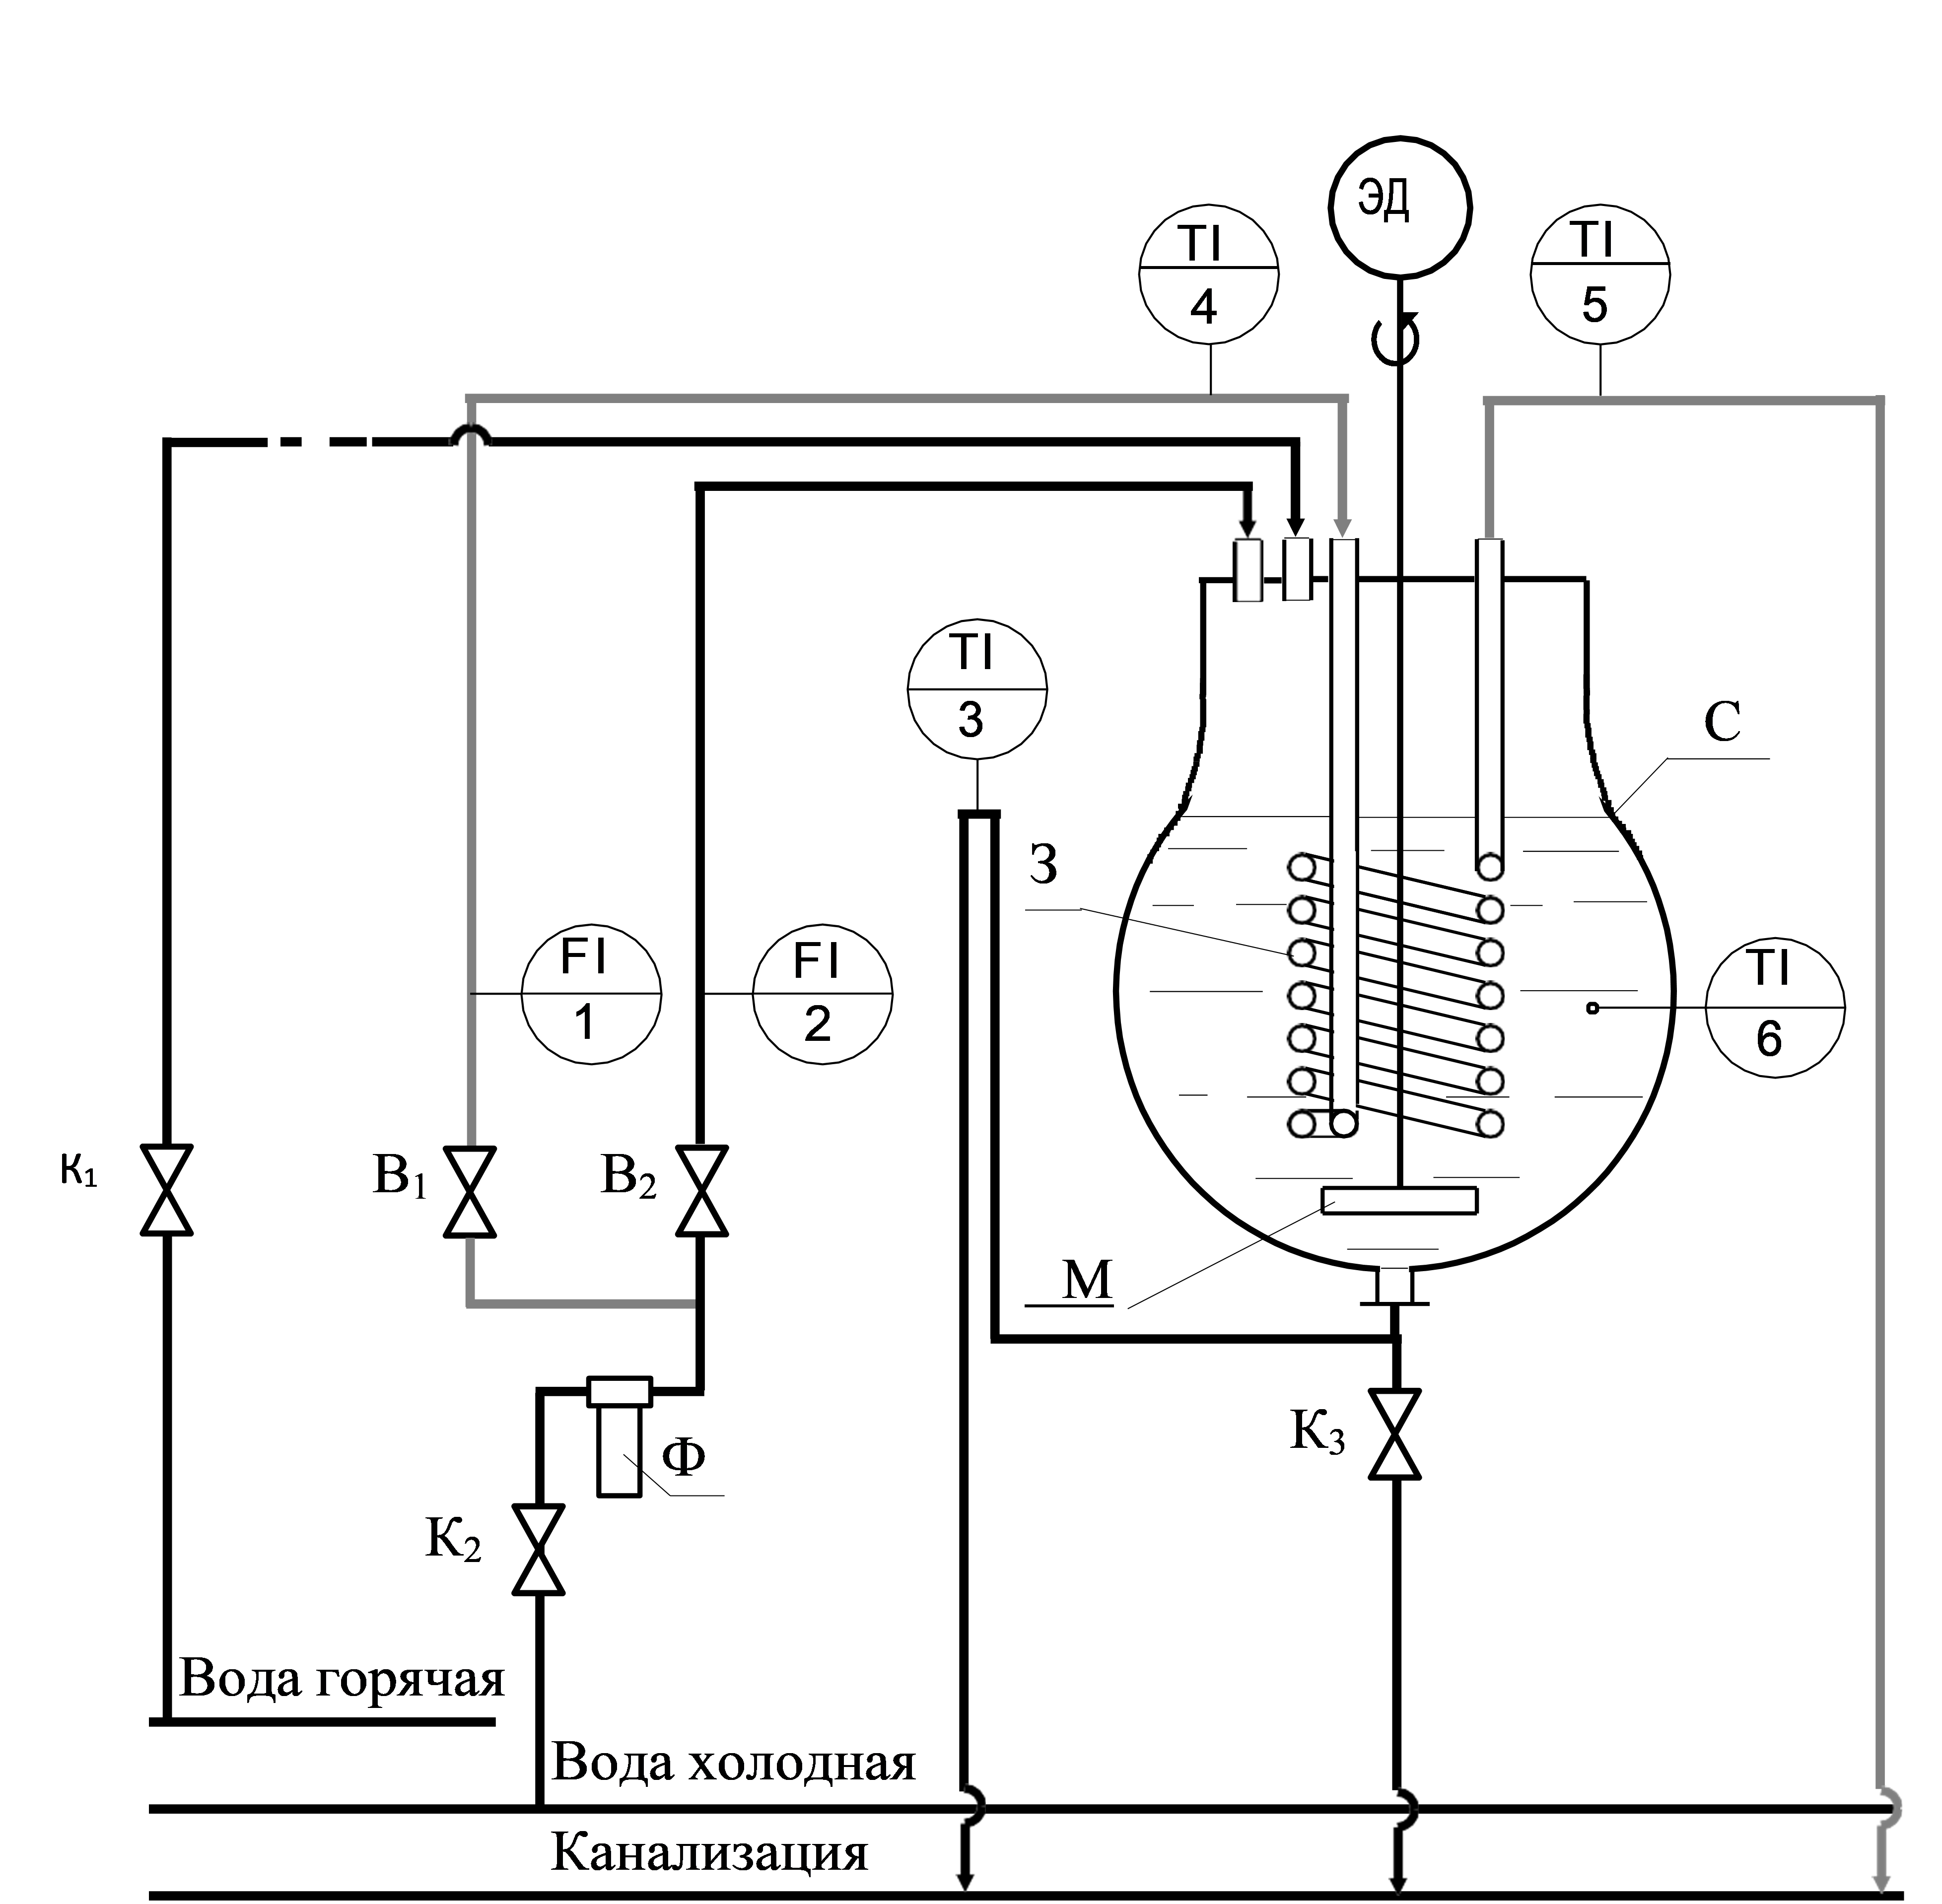
\includegraphics[width=0.6\textwidth]{img/schema.png}~
    \caption{Схема установки}
\end{figure}

Основным элементом установки является стеклянный реакционный сосуд С грушевидной формы.\\

Благодаря специально организованному стоку воды через гидравлический затвор, объём жидкости в заполненном аппарате постоянен и равен $V_C = 24,57$ дм$^3$.
Средний диаметр заполненной части сосуда составляет $D_c = 0,292$ м.\\


Сосуд снабжён змеевиком З, изготовленным из стеклянной трубки размером {\diameter} 18,2 $\times$ 1,8 мм; диаметр витка змеевика $D_{\textrm{вит}} = 172,5$ мм. 
Площадь поверхности погруженной части змеевика, определённая по 
наружному размеру трубки $A = 0,405$ м$^2$. 
Боросиликатное стекло, из которого выполнен змеевик, имеет теплопроводность  ${\lambda}_{CT}$ = 1,14 Вт/(м K).\\

В змеевик может быть подана из водопровода холодная вода, протекающая через фильтр $\Phi$. Расход воды регулируется вентилем $В_1$ и измеряется ротáметром (поз. 1), имеющим на поверхности трубки шкалу, отградуированную в «л/мин» («LPM»).\\

Аппарат снабжён стеклянной лопастной мешалкой М диаметром $d_{M} = 136$ мм, 
вращаемой электродвигателем ЭД. Частота вращения мешалки $n = 2c^{-1}$.

Лабораторная установка оборудована электронными термометрами
(поз. 4, 5), установленными соответственно на линии подачи холодной воды и на линии выхода воды из змеевика. Температура в объёме сосуда измеряется ртутным термометром (поз. 6).


\newpage
\begin{center}
\subsection*{Обработка экспериментальных данных}
\end{center}

Экспериментальные данные используются для расчёта среднего значения коэффициента теплопередачи за период охлаждения и для расчёта
теоретического времени охлаждения жидкости при нестационарном теплообмене.
\begin{table}[!h]
\caption{Экспериментальные данные.}
\begin{center}
\begin{tabular}{|| c | c | c | c | c | c || c | c | c | c | c | c||} 
\hline $i$ & t, \textrm{мин} & 5, \textcelsius & 8, \textcelsius & $6^{*}$, \textcelsius & 6, \textcelsius & $i$ & t, \textrm{мин} & 5, \textcelsius & 8, \textcelsius & $6^{*}$, \textcelsius & 6, \textcelsius\\ [0.5ex] 
 \hline\hline
 0 & 0 & 13,5 & 25,2 & 50,8 & 44,9 & 20 & 10 & 6,3 & 28,1 & 50,9 & 43,5\\ 
 \hline
 1 & 0,5 & 11,6 & 33,8 & 50,8 & 46,1 & 21 & 10,5 & 6,3 & 28,1 & 51,1 & 42,8\\
 \hline
 2 & 1 & 8,2 & 33,6 & 51,1 & 46,6 & 22 & 11 & 6,3 & 28,0 & 51,1 & 43,1\\
 \hline
 3 & 1,5 & 7,1 & 29,7 & 51,1 & 46,2 & 23 & 11,5 & 6,3 & 27,9 & 51,2 & 42,8\\
 \hline
 4 & 2 & 6,5 & 27,9 & 51,3 & 45,5 & 24 & 12 & 6,3 & 27,7 & 51,2 & 42,6\\ 
 \hline
 5 & 2,5 & 6,5 & 27,3 & 51,3 & 44,9 & 25 & 12,5 & 6,3 & 27,6 & 51,3 & 42,3\\
 \hline
 6 & 3 & 6,4 & 26,7 & 51,5 & 43,9 & 26 & 13 & 6,4 & 27,4 & 51,3 & 42,1\\
 \hline
 7 & 3,5 & 6,3 & 26,5 & 51,1 & 43,9 & 27 & 13,5 & 6,4 & 27,2 & 51,3 & 41,9\\
 \hline
 8 & 4 & 6,2 & 26,3 & 50,7 & 43,4 & 28 & 14 & 6,4 & 27,1 & 51,2 & 41,8\\
 \hline
 9 & 4,5 & 6,2 & 26,0 & 50,6 & 43,1 & 29 & 14,5 & 6,4 & 27,0 & 51,1 & 41,6\\
 \hline
 10 & 5 & 6,1 & 25,9 & 50,5 & 42,7 & 30 & 15 & 6,4 & 26,8 & 51,1 & 41,4\\
 \hline
 11 & 5,5 & 6,2 & 25,8 & 50,7 & 42,4 & 31 & 15,5 & 6,3 & 26,7 & 51,0 & 41,3\\
 \hline
 12 & 6 & 6,2 & 25,7 & 50,6 & 42,1 & 32 & 16 & 6,3 & 26,6 & 51,0 & 41,1\\
 \hline
 13 & 6,5 & 6,2 & 25,6 & 50,8 & 41,9 & 33 & 16,5 & 6,3 & 26,6 & 51,0 & 41,0\\
 \hline
 14 & 7 & 6,2 & 25,6 & 50,6 & 41,7 & 34 & 17 & 6,2 & 26,5 & 51,2 & 40,9\\
 \hline
  15 & 7,5 & 6,2 & 25,5 & 50,8 & 41,4 & 35 & 17,5 & 6,3 & 26,5 & 51,2 & 40,8\\
 \hline
  16 & 8 & 6,3 & 25,4 & 50,7 & 41,3 & 36 & 18 & 6,2 & 26,4 & 51,1 & 40,7\\  
 \hline
  17 & 8,5 & 6,2 & 25,7 & 50,8 & 42,4 & 37 & 18,5 & 6,3 & 26,3 & 51,0 & 40,6\\  
 \hline
  89 & 9 & 6,3 & 27,4 & 50,7 & 43,4 & 38 & 19 & 6,3 & 26,3 & 51,0 & 40,6\\  
 \hline
  19 & 9,5 & 6,3 & 28,0 & 50,8 & 43,6 & 39 & 19,5 & 6,3 & 26,1 & 51,1 & 40,5\\ 
 \hline
  20 & 10 & 6,3 & 28,1 & 50,9 & 43,5 & 40 & 20 & 6,3 & 26,1 & 51,0 & 4,0\\\hline
\end{tabular}
\end{center}
\end{table}

\begin{table}[htbp]
\caption{Средние температуры за период охлаждения}
\begin{center}
\begin{tabular}{| c | c | c | c |}
 \hline
5, \textcelsius & 8, \textcelsius & $6^{*}$, \textcelsius & 6, \textcelsius \\
 \hline
6,7 & 27,1 & 51,0 & 41,7 \\
  \hline
\end{tabular}
\end{center}

\end{table}
%
\begin{figure}[h]
    \centering
    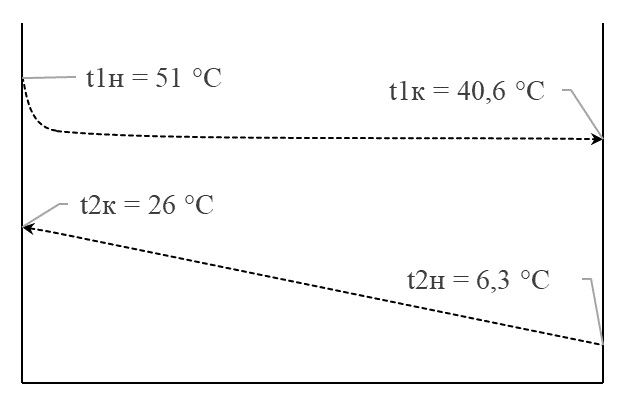
\includegraphics[width=0.4\textwidth]{img/graph.jpg}~
    \caption{Профиль температур теплоносителей}
\end{figure}
\newpage
\begin{center}
\subsubsection*{Расчёты}
\end{center}
Большее и меньшее значение движущей силы:\\
$$\Delta t_{\textrm{м}} = t_{\textrm{1н}} - t_{\textrm{2к}} = 51,0 - 26,1 = 14,5 \; \textrm{К}$$
$$\Delta t_{\textrm{б}} = t_{\textrm{1к}} - t_{\textrm{2н}} = 40,6 - 6,3 = 34,3\;  \textrm{K
}$$

\begin{flushleft}
Среднее логарифмическое значение движущей силы: \\
\end{flushleft}
$$\Delta t_{\textrm{ср}} = \frac{{\Delta t_{\textrm{б}}} - {\Delta t_{\textrm{м}}}}{\ln\left({\dfrac{\Delta t_{\textrm{б}}}{ \Delta t_{\textrm{м}}}}\right)} = \frac{34,3 - 14,5}{\ln\left(\dfrac{34,3}{14,5}\right)} = 23,0 \; \textrm{К}$$

\begin{flushleft}
Среднее значение температуры:
\end{flushleft}
$$t_{\textrm{ср1}} = \frac{t_{\textrm{1н}} + t_{\textrm{1к}}}{2} = \frac{51,6 + 40,8}{2} = 45,8 \; ^\circ \textrm{С}$$
$$t_{\textrm{ср2}} = \frac{t_{\textrm{2к}} + t_{\textrm{2н}}}{2} = \frac{26,1 + 6,3}{2} =  16,2\; ^\circ \textrm{С}$$

\begin{flushleft}
Теплоёмкость теплоагента и хладоагента при средней арифметической температуре:
\end{flushleft}
$$c_{1} = 4179,6 \; \frac{\textrm{Дж}}{\textrm{Кг}  \cdot \textrm{К}} \quad c_{2} = 4184,5 \; \frac{\textrm{Дж}}{\textrm{Кг}  \cdot \textrm{К}}$$

\begin{flushleft}
Объёмные расходы теплоносителей:
 \end{flushleft}
\begin{center}
Расход хол. 3,5 л/мин и тепл. 4 л/мин 
\end{center}
$$\dot{v}_{1} = \frac{4 }{1000 \cdot 60} = 6,667 \cdot 10^{-5} \; \frac{\textrm{м}^3}{\textrm{с}} \quad \dot{v}_{2} = \frac{3,5 }{1000 \cdot 60} = 5,85 \cdot 10^{-5} \; \frac{\textrm{м}^3}{\textrm{с}}$$ 

\begin{flushleft}
Массовые расходы теплоносителей:
\end{flushleft}
$$\dot{m}_{1} = \dot{v}_{1} \cdot \rho_{\textrm{1н}} =  6,667 \cdot 10^{-5} \cdot 987,6 = 6,584 \cdot 10^{-2} \; \frac{\textrm{Кг}}{\textrm{с}}$$
$$\dot{m}_{2} = \dot{v}_{2} \cdot \rho_{\textrm{2н}} =  5,85 \cdot 10^{-5} \cdot 999,9 = 5,849 \cdot 10^{-2} \; \frac{\textrm{Кг}}{\textrm{с}}$$

\begin{flushleft}
Количество теплоты, отдаваемой в единицу времени горячим теплоносителем:
\end{flushleft}
$$Q_{1} = \dot{m}_{1} \cdot c_{1} \cdot \left(t_{\textrm{1н}} - t_{\textrm{1к}} \right) = 6,584 \cdot 10^{-2} \cdot 4179,6 \cdot \left(51,0 - 40,6 \right) = 2862 \; \textrm{Вт}$$

\begin{flushleft}
Количество теплоты, воспринимаемой в единицу времени холодным теплоносителем:
\end{flushleft}
$$Q_{2} = \dot{m}_{2} \cdot c_{2} \cdot \left(t_{\textrm{2к}} - t_{\textrm{2н}} \right) = 5,849 \cdot 10^{-2} \cdot 4184,5 \cdot \left(26,1 - 6,3 \right) = 4846 \; \textrm{Вт}$$

\begin{flushleft}
Экспериментальные значения коэффициента теплопередачи:
\end{flushleft}
$$K_{\textrm{эксп1}} = \frac{Q_{1}}{A \cdot \Delta t_{\textrm{ср}}} = \frac{2862}{0,405 \cdot 23,0} = 307 \; \frac{\textrm{Вт}}{\textrm{м}^2 \cdot \textrm{К}}$$
$$K_{\textrm{эксп2}} = \frac{Q_{2}}{A \cdot \Delta t_{\textrm{ср}}} = \frac{4846}{0,405 \cdot 23,0} = 520 \; \frac{\textrm{Вт}}{\textrm{м}^2 \cdot \textrm{К}}$$

Где $A$ -- площадь поверхности погружённой части змеевика, $A = 0,405$ м$^2$.


\begin{flushleft}
В данной лабораторной работе:
\end{flushleft}
$$t_{\textrm{ср1}} = t_{\textrm{1к}} = 40,6 \; ^\circ \textrm{С}$$
$$t_{\textrm{ср2}} = t_{\textrm{ср1}} - \Delta t_{\textrm{ср}} = 45,8 - 23,0 = 17,603 \; ^\circ \textrm{С}$$

\begin{flushleft}
Физические свойства теплагента и хлдагента при его средней интегральной
температуре $t_{\textrm{ср1}}$ : \\

плотность : $\rho_{1} = 992,0 \; \textrm{Кг}/{\textrm{м}^{3}}, \quad \rho_{2} = 998,0 \; \textrm{Кг}/{\textrm{м}^{3}}$\\
вязкость : $\mu_{1} = 0,6459 \cdot 10^{-3} \; \textrm{Па} \cdot \textrm{с}, \quad \mu_{2} = 1,065 \cdot 10^{-3} \; \textrm{Па} \cdot \textrm{с}$\\
теплоёмкость : $\textrm{с}_1 = 4178,7 \; \textrm{Дж} / \left(\textrm{Кг} \cdot \textrm{К}\right), \quad \textrm{с}_2 = 4183,3 \; \left(\textrm{Дж} / \textrm{Кг} \cdot \textrm{К}\right)$\\
теплопроводность : $ \lambda_1 = 0,621 \; \textrm{Вт} / \left(\textrm{м}^2 \cdot \textrm{К}\right), \quad \lambda_2 = 0,5947 \; \left(\textrm{Вт} / \textrm{м}^2 \cdot \textrm{К}\right)$
\end{flushleft}

\begin{flushleft}
Критерий (число) Прандтля для теплоагента и хладагента: 
\end{flushleft}
$$ Pr_1 = \frac{\textrm{с}_1 \cdot \mu_1}{\lambda_1} = \frac{4178,7 \cdot 0,6459 \cdot 10^{-3}}{0,621} = 4,346$$
$$ Pr_2 = \frac{\textrm{с}_2 \cdot \mu_2}{\lambda_2} = \frac{4183,3 \cdot 1,065 \cdot 10^{-3}}{0,5947} = 7,482$$

\begin{flushleft}
Критерий (число) Рейнольдса теплоагента:
\end{flushleft}
$$Re_1 = \frac{v_1 \cdot {d_{\textrm{м}}^2 \cdot \rho_1}}{\mu_1} = \frac{2 \cdot 0,136^2 \cdot 992,0}{0,6459 \cdot 10^{-3}} = 5,681 \cdot 10^4$$
Где $d_{\textrm{м}}$ диаметр лопастной мешалки  $d_{\textrm{м}} = 0,136$ м, $v_1$ скорость течения теплагента $v_1 = 2 \; \dfrac{\textrm{м}}{\textrm{с}}$.

\begin{flushleft}
Критерий (число) Рейнольдса хладоагента:
\end{flushleft}
$$Re_2 = \frac{v_2 \cdot {d_{\textrm{вн}}^2 \cdot \rho_2}}{\mu_2} = \frac{0,35 \cdot 0,0146^2 \cdot 998,0}{1,065 \cdot 10^{-3}} = 4,79 \cdot 10^3$$
Где $d_{\textrm{вн}}$ внутреный диаметр змеевика $d_{\textrm{вн}} = 0,0146$ м/с, $v_2$ скорость течения теплагента в трубе с внутреным диаметром $d_{\textrm{вн}}\;$, $v_2 = \dot{m_2}/\left(\rho_2 \cdot S_2\right) = 0,35\; \dfrac{\textrm{м}}{\textrm{с}}$.

\begin{flushleft}
Критерий (число) Нуссельта для теплоагента:
\end{flushleft}
$$Nu_1 = 0,87 \cdot {Re_1}^{0,62} \cdot {Pr_1}^{0,33} \cdot \Gamma = 0,87 \cdot 56810^{0,62} \cdot 4,346^{0,33} \cdot 0,466 = 583$$
Г расчитать по формуле $\Gamma = d_{\textrm{м}} / D_c = 0,466$ 
\newpage

\begin{flushleft}
Критерий (число) Нуссельта для хладоагента:
\end{flushleft}

\begin{center}
Как $13,5 \left(\dfrac{d_{\textrm{вн}}}{D_{\textrm{вит}}}\right)^{-0,5} < Re_2 < 18500 \left(\dfrac{d_{\textrm{вн}}}{D_{\textrm{вит}}}\right)^{0,28}$
\end{center}
$$Nu_2 = 0,0575 \cdot {Re_2}^{0,75} \cdot {Pr_2}^{0,45} \left(\dfrac{d_{\textrm{вн}}}{d_{\textrm{вит}}}\right)^{0,28}$$
$$Nu_2= 0,0572 \cdot 4790^{0,75} \cdot 7,482^{0,43} \left(\frac{0,0146}{0,1725}\right)^{0,28} = 46,856$$

\begin{flushleft}
Коэффициент теплоотдачи от теплоагента к стенке:
\end{flushleft}
$$\alpha_1 = \dfrac{Nu_1 \cdot \lambda_1}{d_{\textrm{м}}} = \dfrac{583 \cdot 0,621}{0,136} = 2,664 \cdot 10^3 \; \dfrac{\textrm{Вт}}{\textrm{м}^2 \cdot \textrm{К}}$$

\begin{flushleft}
Коэффициент теплоотдачи от стенки к хладоагенту:
\end{flushleft}
$$\alpha_2 = \dfrac{Nu_2 \cdot \lambda_2}{d_{\textrm{вн}}} = \dfrac{46,856 \cdot 0,5947}{0,0146} = 1,909 \cdot 10^3 \; \dfrac{\textrm{Вт}}{\textrm{м}^2 \cdot \textrm{К}}$$

\begin{flushleft}
Коэффициент теплопередачи, отнесённый к единице
площади наружной поверхности теплообменной трубы:
\end{flushleft}
$$\textrm{К}_{\textrm{Т}} = \left[ \dfrac{1}{\alpha_{1}} + \dfrac{d_{\textrm{н}}}{2\; \lambda_{\textrm{ст}}} \cdot \ln \left( \dfrac{d_{\textrm{н}}}{d_{\textrm{вн}}} \right) + \dfrac{1}{\alpha_{2}} \cdot \dfrac{d_{\textrm{н}}}{d_{\textrm{вн}}} \right]^{-1}$$
$$\textrm{К}_{\textrm{Т}} = \left[\dfrac{1}{2664} + \dfrac{0,0182}{2 \cdot 1,14} \cdot \ln \left(\dfrac{0,018}{0,0146} \right) + \dfrac{1}{1909} \cdot \dfrac{0,0182}{0,0146} \right]^{-1} = 370 \; \dfrac{\textrm{Вт}}{\textrm{м}^2 \cdot \textrm{К}}$$\\


\begin{center}
\subsection*{Заключение}
\end{center}

В ходе лабораторной работы мы провели стационарный теплообмен и рассчитали коэффициент теплопередачи, который составил 370,44 $\textrm{Вт}/\left(\textrm{м}^2 \cdot \textrm{К}\right)$.



\end{document}
%\usepackage[english,russian]{babel}